\documentclass[11pt]{article}
\usepackage{graphicx}    % needed for including graphics e.g. EPS, PS
\topmargin -1.5cm        % read Lamport p.163
\oddsidemargin -0.04cm   % read Lamport p.163
\evensidemargin -0.04cm  % same as oddsidemargin but for left-hand pages
\textwidth 16.59cm
\textheight 21.94cm 
%\pagestyle{empty}       % Uncomment if don't want page numbers
\parskip 7.2pt           % sets spacing between paragraphs
%\renewcommand{\baselinestretch}{1.5} % Uncomment for 1.5 spacing between lines
\parindent 0pt		 % sets leading space for paragraphs

\begin{document}         
% Start your text

\section{Abstract}
\label{Abstract}
Stacked de-noising auto-encoders (SdAs) have shows excellent performance on machine perception tasks. In this paper I test the algorithm on a planning task, the game of Go. If it performs better than a flat network, then I believe that it lends strength to the hypothesis that SdAs are a good model of how the neocortex learns. The neocortex has a uniform structure throughout, yet it has high plasticity and performs perception, motor-control, and high-level planning with seemingly the same mechanism. I use one possible unification of the process of perception and control to make an SdA play Go. I train the network to form a hierarchical model of a dataset of several thousand completed go games, and I interpret it's expectations as plans. The network preferentially remembers games from the perspective of the winning player. This is based on the hypothesis that the self-serving bias observed in psychology is an artifact of the unification of perception and control.

\section{Introduction}
\label{Introduction}

\section{0.0 Background on de-noising autoencoders}
\label{Background on de-noising autoencoders}
Autoencoders, or autoassociators as they are sometimes called, are a variant of the simple three-layer artificial neural network where the output is expected to equal the input and the hidden layer is smaller or sparser than than the input layer. An autoencoder takes an input $\mathbf x\in[0,1]^d$ and first maps it (with an encoder) to a hidden representation $\mathbf y\in[0,1]^{d'}$ through a deterministic mapping, e.g.:
\[
\mathbf y = s(\mathbf W\mathbf x + \mathbf b)
\]
Where $s$ is a non-linearity such as the sigmoid. The latent representation $\mathbf y$, or code is then mapped back (with a decoder) into a reconstruction $\mathbf z$ of same shape as $\mathbf x$  through a similar transformation, e.g.:
\[
\mathbf z = s(\mathbf W'\mathbf y + \mathbf b')
\]
$\mathbf z$ should be seen as a prediction, or {\it reconstruction}, of  $\mathbf x$ given the code  $\mathbf y$. The parameters of this model ($\mathbf W$, $\mathbf W'$, $\mathbf b$, and $\mathbf b'$) are optimized such that the average reconstruction error is minimized\cite{Bengio09}.

Show figure to explain

The aim of the autoencoder to learn the code $\mathbf y$ a distributed representation that captures the coordinates along the main factors of variation in the data (similarly to how principal component analysis (PCA) captures the main factors of variation in the data). Because $\mathbf y$ is viewed as a lossy compression of $\mathbf x$, it cannot be a good compression (with small loss) for all $\mathbf x$, so learning drives it to be one that is a good compression in particular for training examples, and hopefully for others as well, but not for arbitrary inputs. That is the sense in which an auto-encoder generalizes: it gives low reconstruction error to test examples from the same distribution as the training examples, but generally high reconstruction error to uniformly chosen configurations of the input vector.

If there is one linear hidden layer (the code) and the mean squared error criterion is used to train the network, then the  hidden units learn to project the input in the span of the first  principal components of the data. If the hidden layer is non-linear, the auto-encoder behaves differently from PCA, with the ability to capture multi-modal aspects of the input distribution. The departure from PCA becomes even more important when we consider stacking multiple encoders (and their corresponding decoders) when building a deep auto-encoder [Hinton06].

Explain the necessity of sparsity using the notion of data compression. Cite the evidence that the brain uses sparse representations. 

The auto-encoder alone is not sufficient to be the basis of a deep architecture because it has a tendency towards over-fitting. The denoising autoencoder (dA) is an extension of a classical autoencoder introduced specifically as a building block for deep networks\cite{Vincint08}.  It attempts to re-construct a corrupted version of the input. The error in $\mathbf z$ is still compared against the un-corrupted input. The stochastic corruption process consists in randomly setting some of the inputs (as many as half of them) to zero. Hence the denoising auto-encoder is trying to predict the corrupted (i.e. missing) values from the uncorrupted (i.e., non-missing) values, for randomly selected subsets of missing patterns. This modification allows the dA to generalize well and produces compounding benefits when the dA's are stacked into a deep network\cite{Hinton06}. Hinton(google tech talk 3) suggests that the stochastic timing of the action potentials observed in neurons is a similar feature evolved to alleviate this problem of over-fitting.

\section{0.1 Stacked de-noising autoencoders}
\label{Stacked de-noising autoencoders}
Stacked denoising autoencoders, abbreviated SdA to differentiate them from other learning algorithms with that acronym, are not just neural networks with additional hidden layers, but a structure with individual levels of simple three-layer denoising autoencoders. First, a single denoising autoencoder is trained on the data. It's hidden layer converges on a sparse distributed representation of the training set. This essentially replaces the step where a researcher would have to design a collection of good features. Then, a second denoising autoencoder is trained to reconstruct corrupted versions of the activation of the hidden layer of the first dA for the collection of training examples. (the first level does not learn during this time). After a sufficient number of levels have been added, if the network is to be used for classification, the encoders and decoders from each level are assembled into one long network and fine-tuned using back-propagation.

\begin{figure}[htb]
\begin{center}
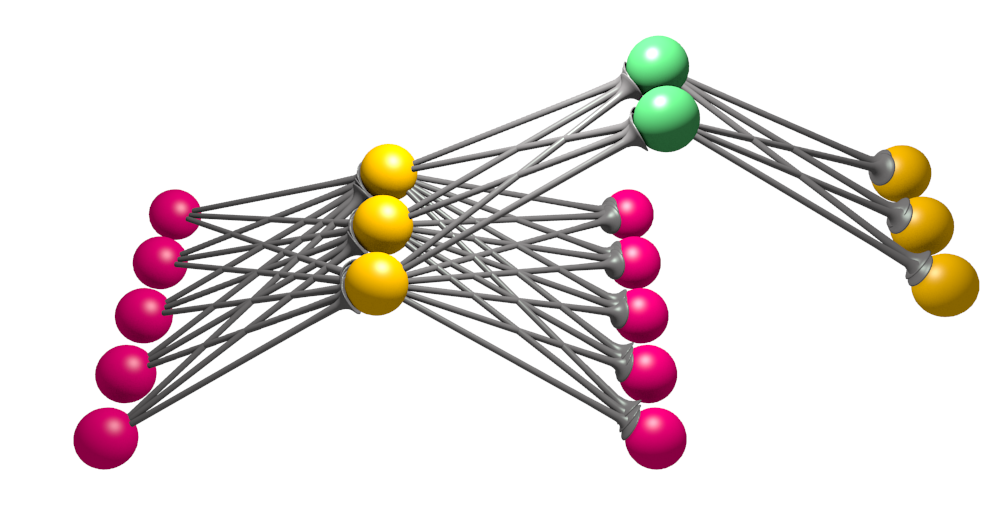
\includegraphics[height=2.585in,width=5in]{sda_fig}
\caption{An SdA with two autoencoders. Each autoencoder is a a simple three layer network. The input/output to the first layer is the pink level, and the yellow level is it's distributed code, or hidden layer. The yellow hidden layer is then used as input/output to another autoencoder, it's hidden layer is shown in green.}
\end{center}
\end{figure}

Explain the necessity of a deep network and the curse of dimensionality.

Cite the many new developments in the field of deep nets.

Stacked denoising autoencoders are more complex neural networks, who's basic component are a variant of simple, three-layer networks. The are still simple compared to the neocortex, but have some of the same performance characteristics. The neocortex has several layers, but those layers do not correspond to the layers of the stack in a stacked denoising neural autoencoder. An SdA only models the lateral connections that pyramidal cells make between areas of the cortex. Each pyramidal cell is a sort of representative for around 10,000 other neuron's in it's vicinity.  For example, the areas V1 through V4 in the visual cortex are organized in a functional hierarchy, but they are not in a physical stack of levels. Pyramidal cells make lateral connections between the levels, which are arranged laterally, within the sheet of the neocortex.

Note that I am using the word 'layer' to refer to the three layers in a single dA, and the word 'level' to refer to the dA's within an SdA.

\section{1.0 Successes of SdAs on machine perception tasks}
\label{Successes of SdAs on machine perception tasks}

Tell the story of Hinton's grad student who kept adding another layer, and cite the proof of the increase in the upper bound on prediction accuracy.

Cite Hinton's work on images, video, sound, and mocap.

The largest experiment so far with an SdA, by Google, was able to learn feature detectors for the human face, and a cat, among other things, by training on 10 millions images taken from youtube videos\cite{Le12}. They used 9 levels of autoencoders. Some other tweaks were used as well, such as local contrast normalization (which basically saves them a level) and Max pooling, a standard procedure in machine vision. They trained the network for three days on a cluster with computing power in the neighborhood of 1 PFLOP. This image broke out on reddit with the title "first machine forms concept on it's own". While that's an oversimplification, and it's not the first, it is essentially what Google set out to do.

This appears to be a white white male human face, and the fact that it was selected by the researches probably reflects their own bias, and does not preclude that the SdA also arrived at codes for black, female, child, elderly, or non-human faces. Although that may not be as efficient as a code which can represent all faces as the sum of a pale white genderless face and some hair and color and eyes. 9 levels up in the hierarchy the categories are very abstract, so this is at least plausible.

\begin{figure}[htb]
\begin{center}
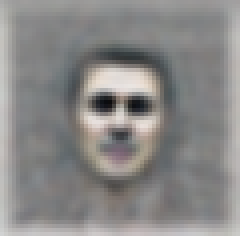
\includegraphics[height=1.6in,width=1.6in]{gman}
\caption{A representation of the face detection feature learned by Google's SdA. This image is generated by computing the input that would maximally activate the hidden node in the top layer that has come to represent faces. The SdA was trained on 10 million 200x200 images from youtube\cite{Le12}.}
\end{center}
\end{figure}



Training neural networks is an easy process to paralellize and distribute across many computers. However, all the extra training that occurs in an SdA requires even more computer power than usual. The de-noising step is essentially just a supersampling step to create more training examples, and adds an order of magnitude or two to the training time. For this reason, and because of falling costs, the latest developments in SdAs have been run on GPUs. Nvidia's CUDA shader language combined with a top of the line GPU (or several) affords 10 to 1000 fold increases in speed for applications which are very paralellizable. Using Python and Theano\cite{Bergstra10}, a binding to the GPU accelerated linear algebra library LAPACK on Ubuntu, and a single Nvidia GTX 570 capable of 1405 GFLOPS, I was able to achieve about 20x increase in speed on a simple SdA pre-training operation on the MINST dataset, over a quad-core Intel i5-2500k CPU at 4.5 Ghz, measured to be capable of only 59 GFLOPS.

\section{1.1 Applications of SdAs to planning tasks}
\label{Applications of SdAs to planning tasks}

The essence of planning is the attainment of a goal through a series of intermediate steps which do not necessarily lead directly toward that goal\cite{Baker95}. Various kinds of advanced neural network based models have been applied to planning tasks, but SdA's are not among them.

Self-Organizing Maps (SOM) were used by Anmin Zhu to control robot swarms. 



\section{2.0 Plausibility of SdA's as a model of the mammalian neocortex}
\label{Plausibility of SdA's as a model of the mammalian neocortex}

The primate visual cortex is one of the best understood brain regions in the animal kingdom. We know that it is composed of several levels, each more abstract than the one before it. The cortical columns in V1 are sensitive to a small receptive field of light coming in from the lateral genticulate cortex, which in turn receives information from the optic nerve. They are each slightly sensitive to certain angles and colors more than others. V2, which has connections drawing from V1 and other areas, has cells that are sensitive to mildly complex shapes somewhat invariant to translation, rotation, and scale, and will detect these shapes within a slightly larger receptive field. This gradual increase in abstraction continues as you move up the chain of levels, until you have neurons that are sensitive to something invariant like "person" or "thing moving towards me at an alarming speed"

The SdA method is evolving with functionality and performance in mind, and not explicitly to mimic the cortex, but we find that it has many of the same strengths and weaknesses. One such strength is it's plasticity. An SdA pre-trained to see video, performed better at a hearing task after fine-tuning, than a randomly initialized network fine-tuned in the same way. This is presumably because sound and video share some macro-statistical properties, such as having a high kurtosis.

An SdA also goes through different phases of learning that resemble the phases in a person's maturation. We know that plasticity in the brain decreases over time, and at about 30, the brain changes over to a new mode where it begins to fine tune existing connections and grows almost no new connections in the cortex.

\section{2.1 Philosophical points}
\label{Philosophical points}

The levels in the SdA are levels of abstraction. What are the implications of a possible root at the top of this tree?

Perception is like nested stack of expectations, specific expectations of the near future based on a deluge of sensory data, and a smaller collection of abstract expectations of the medium range future based on a shower of specific, short-range expectations and some more sensory data. Recurse until lost.

Does this tree have a root? is there some "most abstract representation" of our sensory experience that we can expect in the indefinitely long run, that decodes to the specifics that we will in fact observe from this point on? I think that this very theory is a candidate. But that's not as important as it sounds. What any abstract expectation actually predicts depends on the more specific models below it, and the sensory data yet to be observed.  "This too shall pass" would make a perfectly good root for our tree, if giving it that role didn't actually turn it into a paradox. A root here is really not more important than a leaf.

Let me re-iterate. I am operating on the assumption for this project, that perception and planning are both part of the same process, so the most abstract representations are joint models of sensory experience and action. The model of sensory data is influenced by three main factors. The accuracy, the sparsity, and the desirability, or pleasurableness to the creature. At all levels, the representations which jointly satisfy these three metrics come to dominate. In the case of a game this last factor would be the points or wins/losses experienced by the player. The player perceives the state of the game and the state of it's own recent actions, and expects a likely, sparse, and desirable scenario next, and then is made to take any actions it expected of itself which are legal in the rules of the game. It may not be the most brilliant way to play a game, but I think It would at least perform OK at Puerto Rico, a game about economic growth.

Jeff Hawkins said in 2004, Neural networks were a genuine improvement of the AI approach because their architecture is based, though very loosely, on real nervous systems...But as the neural network phenomenon exploded on the scene, it mostly settled on the class of ultra-simple models that didn't meet any of [his criteria for biological plausibility]. Most neural networks consisted of a small number of neurons connected in three rows...I thought the field would quickly move on to more realistic networks, but it didn't. Because these simple neural networks were able to do interesting things, research seemed to stop there for years. \cite{Hawkins04}

\section{3.0 Expected performance of SdA vs. dA}
\label{Expected performance of SdA vs. dA}

An experiment where an single de-noising auto-encoder is trained on the full dataset, and a stacked denoising auto-encoder of 4 levels is trained on the same dataset is used to compare the effectiveness of more layers.

simple greedy hill climbing approach

\section{3.1 Implementation of Go Engine}
\label{Implementation of Go Engine}

A standard go engine is a computer program which can speak the go protocol and decide on moves from game states. Through a bit of wrapper code, it connects to a go server like KGS or a local game arbitration software where it plays games against humans or other go engines.


Why was Go chosen?
* it is a difficult game for computers, with a huge branching factor. This ensures that brute force is infeasible and rules out the possibility of it being used in-whole or in-part.
* Go requires planning at different scales of time and space. Sometimes sacrifice is strategic.
* Neither a purely greedy or purely sustainable outlook is as good as a balance between the two.

\section{3.2 Implementation of SdA-based decider}
\label{Implementation of SdA-based decider}

\section{4.0 Performance of SdA-based player against dA player and various other opponents}
\label{Performance of SdA-based player against dA player and various other opponents}

performance matrix?
SdA vs. dA
SdA vs. SdA
SdA vs. me
SdA vs. online players who think they are playing a human. (definitely don't have time to do this)

\section{4.1 Conclusion and lessons learned}
\label{Conclusion and lessons learned}




\begin{thebibliography}{99}

\bibitem{Baker95} S. C. Baker, R. D. Rogers, A. M. Owen, C. D. Frith, R. J. Dolan, R. S. J. Frackowiak, T. W. Robbins. Neural systems engaged by planning: a PET study of the Tower of London task. Neuropsychologia,Vol. 34, No. 6, pp. 515-526, 1996
 
\bibitem{Bengio07} Bengio, P. Lamblin, D. Popovici and H. Larochelle, Greedy Layer-Wise Training of Deep Networks, in Advances in Neural Information Processing Systems 19 (NIPS�06), pages 153-160, MIT Press 2007.
 
\bibitem{Bengio09} Bengio, Learning deep architectures for AI, Foundations and Trends in Machine Learning 1(2) pages 1-127.

\bibitem{Hawkins04} Jeff Hawkins and Sandra Blakeslee. On Intelligence. Times Books, 2004.

\bibitem{Hinton06} G.E. Hinton and R.R. Salakhutdinov, Reducing the Dimensionality of Data with Neural Networks, Science, 28 July 2006, Vol. 313. no. 5786, pp. 504 - 507.

\bibitem{Hinton07} G.E. Hinton, S. Osindero, and Y. Teh, �A fast learning algorithm for deep belief nets�, Neural Computation, vol 18, 2006

\bibitem{Bergstra10} J. Bergstra, O. Breuleux, F. Bastien, P. Lamblin, R. Pascanu, G. Desjardins, J. Turian, D. Warde-Farley and Y. Bengio. �Theano: A CPU and GPU Math Expression Compiler�. Proceedings of the Python for Scientific Computing Conference (SciPy) 2010. June 30 - July 3, Austin, TX

\bibitem{Le12} Quoc Le, Marc'Aurelio Ranzato, Rajat Monga, Matthieu Devin, Kai Chen, Greg Corrado, Jeff Dean, Andrew Ng. Building high-level features using large scale unsupervised learning. International Conference in Machine Learning, 2012.

\bibitem{Ranzato06} Marc�Aurelio Ranzato, Christopher Poultney, Sumit Chopra, and Yann LeCun. Efficient Learning of Sparse Representations with an Energy-Based Model. Advances in Neural Information Processing Systems, 2006.

\bibitem{Seyfarth01}  Seyfarth, Andreas, Puerto Rico Rulebook. Rio Grande Games, 2001

\bibitem{Vincint08} Vincent, H. Larochelle Y. Bengio and P.A. Manzagol, Extracting and Composing Robust Features with Denoising Autoencoders, Proceedings of the Twenty-fifth International Conference on Machine Learning (ICML�08), pages 1096 - 1103, ACM, 2008.
 
\end{thebibliography}
\end{document}








